\documentclass{article}
\usepackage[utf8]{inputenc}
\usepackage{amsmath}      % Gir blant annet muligheten til ligningsreferering med kommandoen \eqref
\usepackage{graphicx}     % Nødvendig for å legge til figurer/bilder
\usepackage{wrapfig}      % For å integrere figurer i tekst
\usepackage{lipsum}       % Gir tilgang til fyll tekst ved kommandoen \lipsum
\usepackage[norsk]{babel} % For å få norsk standard

\title{Latex-kurs med numfys.net}
\author{Eilif Sommer Øyre}
\date{19. september 2019}

\begin{document}

\maketitle

\section{Ligninger}

Ligning inne i en tekst kan skrives mellom to dollartegn: $F = ma$. Ved nummerert ligning på egen linje brukes \LaTeX-miljøet \texttt{\textbackslash begin\{equation\}}.
\begin{equation}
K = \frac{1}{2}mv^2
\end{equation}

For å unngå nummerering kan en bruke \texttt{\$\$ \$\$}
$$ \int_a^b x dx = \frac{1}{2}b^2 - \frac{1}{2}a^2 .$$

Bruk \texttt{\textbackslash label} for å definere et navn å referere til
\begin{equation}
\rho(x) \equiv 9\frac{n^{3/2} \hbar^2}{4\pi \epsilon_0} \Gamma(x)
\label{rho}
\end{equation}

Ligning \eqref{rho} er en tilfeldig definisjon.

\begin{table}[h] % Parameteren "h" står for "here" og ber latex om å plassere figuren der den står i koden (sånn ca.). Bruk "h!" eller "H" for å overstyre automatiske latex funksjoner som flytter på  figurer
\centering
\begin{tabular}{| l | c | r |} % Parameterene "l c r" angir tre kolonner, venstrejuster, sentrert, og høyrejustert, henholdsvis.
\hline % Horisontal strek i tabellen
\multicolumn{3}{|c|}{En enkel tabell} \\ % Slår sammen 3 kolonner til én med sentrert tekst og vertikale linjer på hver side.
\hline
kolonne 1 & kolonne 2 & kolonne 3 \\
\hline
\hline
21 & 22 & 23 \\
31 & 32 & 33 \\
\hline
\end{tabular}
\caption{Dette er en tabelltekst}
\label{tabell:1}
\end{table}


\listoftables
\newpage

\section{Figurer/bilder}
Figur \ref{fig:1} under er laget i vektorgrafikkprogrammet Inkscape.
\begin{figure}[h!] 
\centering
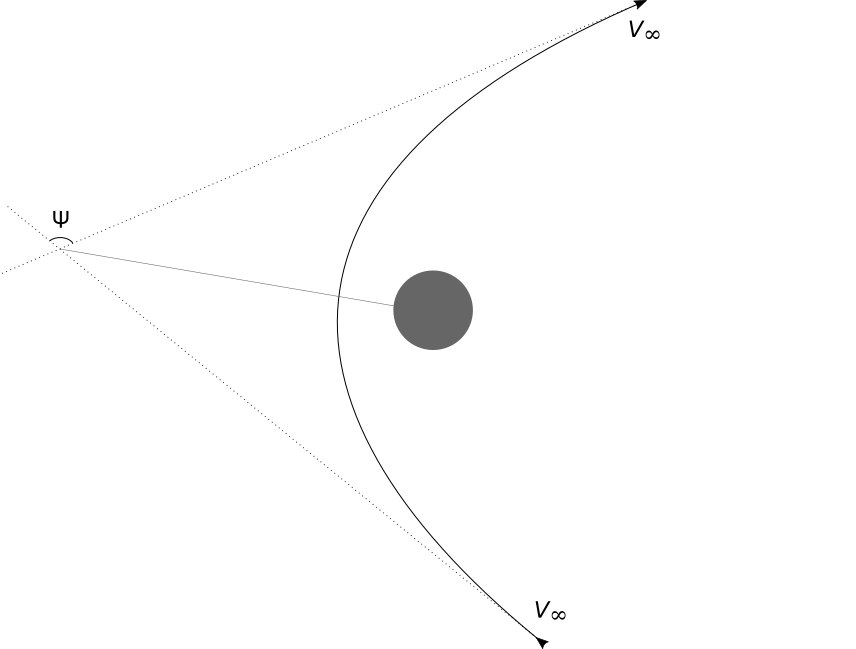
\includegraphics[width=0.8\textwidth]{gravityassist} % Det går også an å definere bredde og høyde til figuren med andre enheter enn \textwidth. F.eks "[width=5cm, height=600mm, angle=45]". I eksemplet har jeg også rotert figuren
\caption{The trajectory of a spaceship passing a planet}
\label{fig:1}
\end{figure}

\begin{wrapfigure}{r}{0.25\textwidth} % "r" gir beskjed at figuren skal være på høyre siden av teksten. "0.25\textwidth" er bredden på plassen teksten skal gi figuren.
\centering % Sentrerer figuren i den angitte plassen
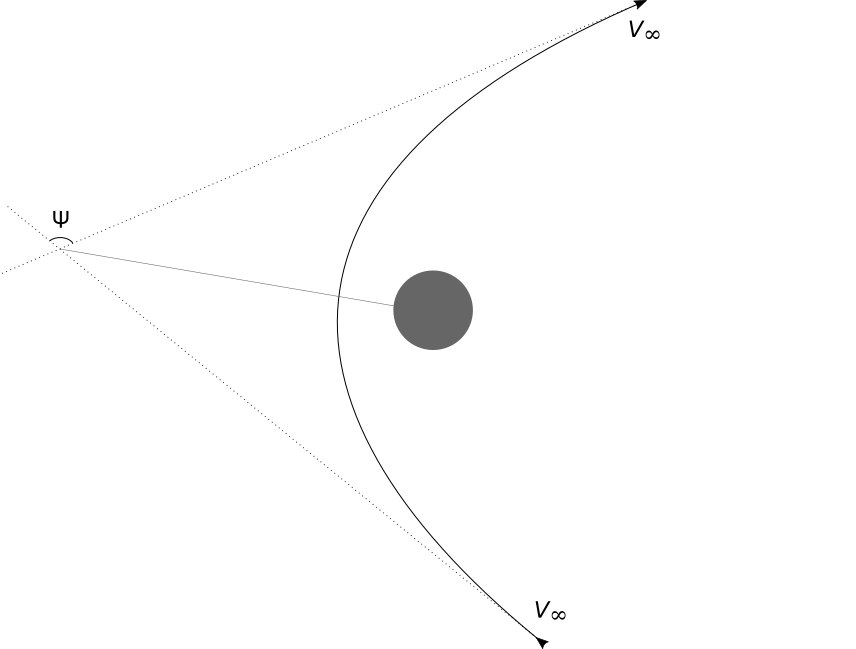
\includegraphics[width=0.25\textwidth]{gravityassist} % Her settes størrelsen på figuren like stor som plassen den har blitt angitt.
\end{wrapfigure}

\lipsum[1] % Fylltekst

\newpage

\section{Referanser}
Se \cite{Sauer} for mange spennende numeriske metoder.
    '
\begin{thebibliography}{10} % Gir plass til 10 kilder
\bibitem{Sauer} 
Timothy Sauer, \textit{Numerical Analysis, second edition}, 2014, Pearson Education Limited.

% Alternativ måte å liste kilder på følger under.
\bibliographystyle{unsrt} % "unsrt" er en spesifik stil referansene. Se https://www.overleaf.com/learn/latex/Bibtex_bibliography_styles for flere stiler
\bibliography{sample} % Denne kommandoen henter så alle referansene lagret i .bib-fila med navn "sample". Referansene i "sample.bib" må skrives i et spesifik format. I tillegg, for at referansene skal bli listet, må de være referert til i teksten ved bruk av \cite{}. 

\end{document}
